\documentclass[a4paper]{article}
\usepackage[14pt]{extsizes} % для того чтобы задать нестандартный 14-ый размер шрифта
\usepackage[left=1.5cm,right=1.5cm,top=2cm,bottom=2cm]{geometry}
\usepackage{multirow}
\usepackage{parallel}
\usepackage {graphicx}
\usepackage{multicol}
\usepackage[utf8x]{inputenc} % указать кодировку русского текста
\usepackage[russian]{babel} % указать, что язык текста - русский
\usepackage{fancyhdr}
\pagestyle{fancy}
\usepackage{graphicx}
\graphicspath{{pictures/}}
\DeclareGraphicsExtensions{.pdf,.png,.jpg, .jpeg}
\usepackage{tocloft}
\usepackage{wrapfig}
\usepackage{tikz}

\usepackage{enumitem}
\setlist[enumerate,itemize]{leftmargin=0pt,itemindent=2.7em}
\renewcommand{\cftsecleader}{\cftdotfill{\cftdotsep}}
\begin{document} 
\large
\noindent \textbf{Лабораторная работа 4.3.2А: Дифракция света на ультразвуковой волне в жидкости}\\
\\
\normalsize
\textbf{М.Шлапак}\\
\line(1,0){18cm}\\
\\
\footnotesize
\textit{Изучено явление дифракции света на синусоидальной акустической решётке, проведено наблюдение фазовой решётки методом тёмного поля.}\\
\\
\textit{\textbf{Ключевые слова:} дифракция света, синусоидальная рещётка, фазовая решётка, метод тёмного поля, скорость ультразвука}\\
\fancyhead[L] {Дифракция света на ультразвуковой волне в жидкости, М.Шлапак}

\begin{multicols}{2}

\begin{enumerate}
\small
\item \textbf{Введение}\\ 
В данной работе опытным путём была измерена скорость ультразвука в воде путём измерений на акустической решетке, попутно был освоен метод тёмного поля - один из методов, помогающих в визуализации фазового объекта. \\
\item \textbf{Теоретические основы}\\
При прохождении ультразвуковой волны через жидкость в ней возникают периодические неоднородности коэффициента преломления, создается фазовая решетка, которую мы считаем неподвижной ввиду малости скорости звука относительно скорости света. Показатель преломления n изменяется по закону:
	\begin{equation}\label{trivial}
	n = n_0 (1 + m \cos \Omega x)
	\end{equation}
	, где $ \Omega = 2 \pi / \Lambda $ --- волновое число для ультразвуковой волны, $ m $ --- глубина модуляции показателя преломления $ n $ $ (m \ll 1 $).\\
Положим фазу $ \phi $ колебаний световой волны на передней стенке кюветы равной нулю, тогда на задней поверхности она равна:
	\begin{equation}\label{}
	\phi  = k n L = \phi_0 (1 + m \cos \Omega x)
	\end{equation}
	, где $ L $ --- толщина жидкости в кювете, $ k = 2 \pi / \lambda $ --- волновое число для света.\\
	После прохождения через кювету световое поле есть совокупность плоских волн, распространяющихся под углами $ \theta $, соответствующими максимумам в дифракции Фраунгофера:\\
\begin{equation}\label{}	
	\Lambda \sin \theta_m = m \lambda
\end{equation}
Этот эффект проиллюстрирован на рисунке 1.
	Зная положение дифракционных максимумов, по формуле (3) легко определить длину ультразвуковой волны, учитывая малость $ \theta $: $ \sin \theta \approx \theta \approx l_m /F  $, где $ l_m $ --- расстояние от нулевого до последнего видимого максимума, $ F $ --- фокусное расстояние линзы. Тогда получим:
	
	\begin{equation}\label{}
	 \Lambda = m \lambda F/ l_m 
	\end{equation}
	Скорость ультразвуковых волн в жидкости, где $ \nu $ --- частота колебаний излучателя:
\begin{equation}\label{}
	v = \Lambda \nu 
\end{equation}
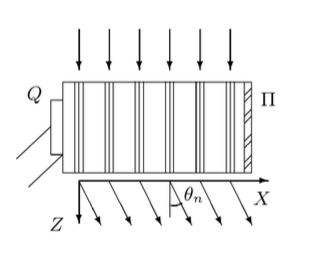
\includegraphics[width=9cm]{1.png}
\textit{рис. 1. Дифракция световых волн на акустической решетке}\\
\item \textbf{Экспериментальная установка}
\begin{enumerate}
\item \textbf{Схема наблюдения дифракции на акустической решётке}\\
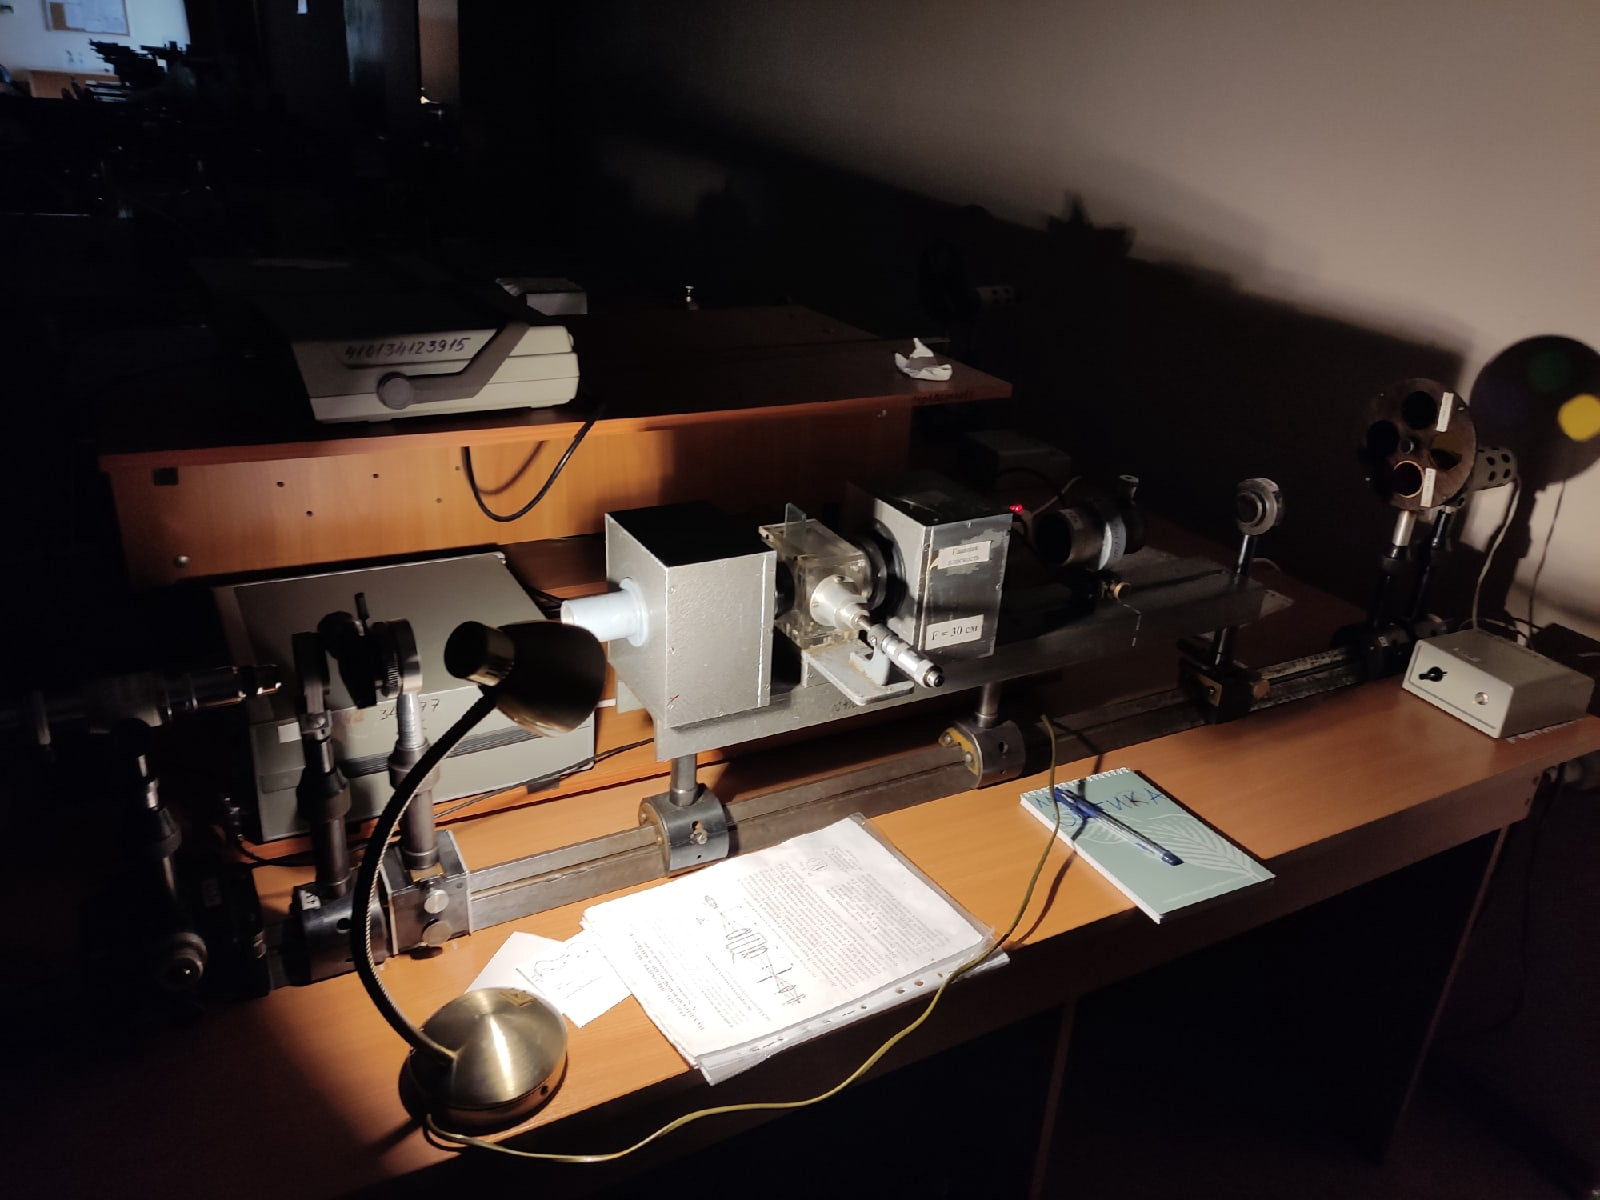
\includegraphics[width=8.5cm]{exp3}\\
\textit{рис.2 Экспериментальная установка}\\
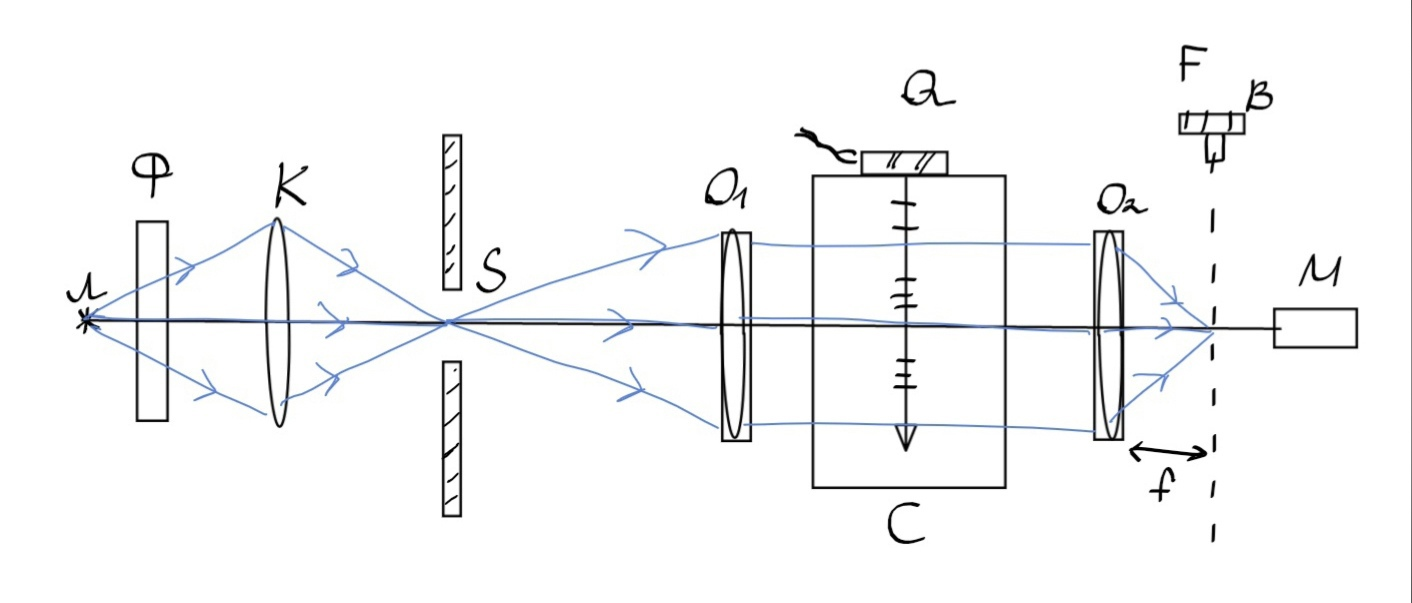
\includegraphics[width=9cm]{exp1}\\
\textit{рис.3 Наблюдение дифракции на акустической решётке}\\
\item \textbf{Наблюдение акустической решетки методом тёмного поля}\\
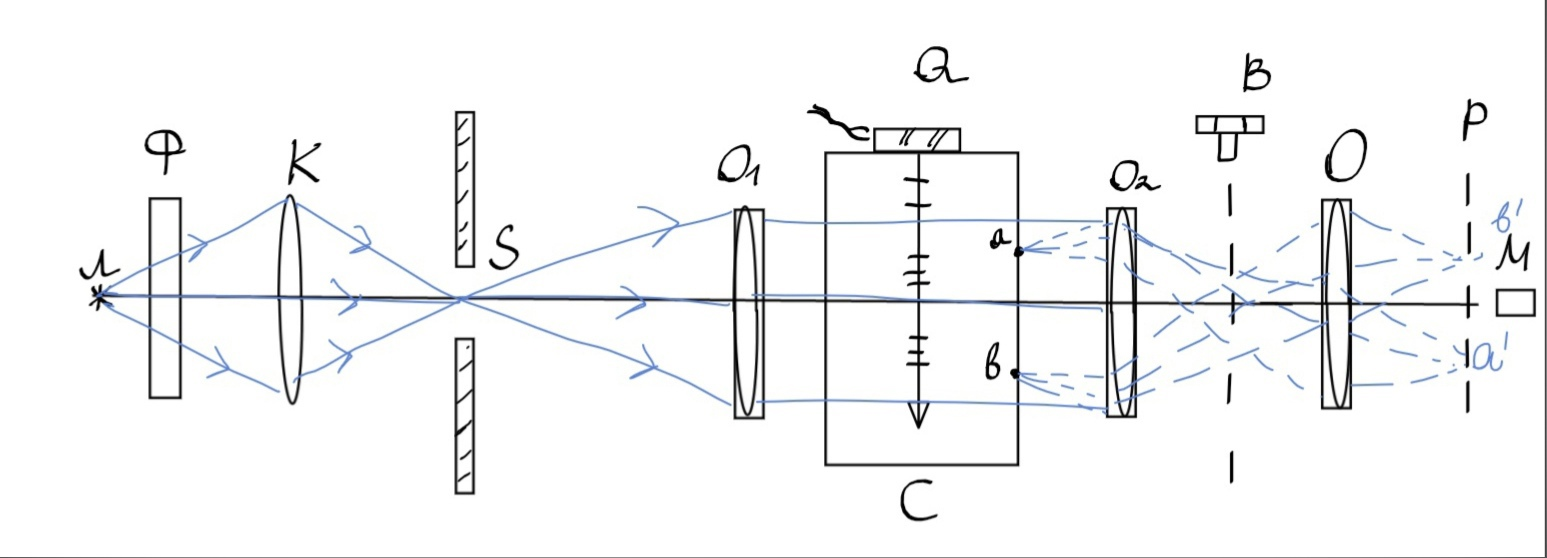
\includegraphics[width=9cm]{exp2}\\
\textit{рис.4 Наблюдение акустической решётки методом тёмного поля}\\
\\
Л - источник света, Ф - светофильтр,К - конденсор, О1 и О2 - объективы, С - кювета, М - микроскоп, О - вспомогательная положителньая линза\\
\end{enumerate}	

\item \textbf{Результаты эксперимента}\\
Запишем начальные данные: $f = 30 \; \textit{см}$, $\lambda = 605 \; \textit{нм}$
\begin{enumerate}
\item \textbf{Определение скрости ультразвука по дифракционной картине}\\
1) После сборки установки и яркого освещения щели с помощью конденсора получим в поле зрения микроскопа систему дифракционных полос.\\
\\
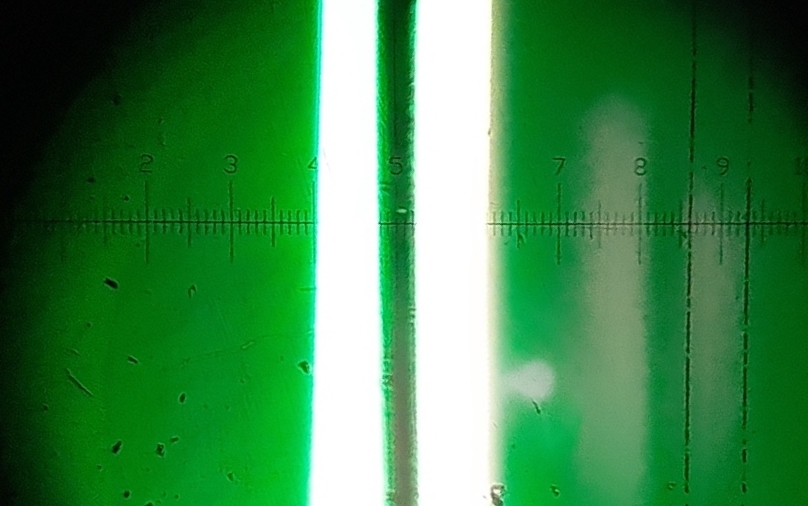
\includegraphics[width=9cm]{exp4}\\
\textit{рис.5 Дифракционные полосы для зелёного светофильтра}\\
\\
2) Заменим широкополосный зелёный фильтр красным и измерим положения $x_m$ дифракционных максимумов с помощью микрометрического винта для трёх частот.\\
2.1) \begin{tabular}{|l|l|l|l|l|l|}
\hline
m & -2 & -1 & 0 & 1 & 2\\
\hline
$x_m$, мкм & 1980 & 1840 & 1720 & 1580 & 1440\\
\hline
\end{tabular}\\
\\
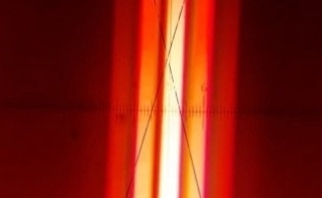
\includegraphics[width=9cm]{exp5}\\
\textit{рис.6 Дифракционная картинка на частоте $\nu = 1,115$ Мгц}\\
\\
2.2) \begin{tabular}{|l|l|l|l|}
\hline
m & -1 & 0 & 1\\
\hline
$x_m$, мкм & 1900 & 1720 & 1540\\
\hline
\end{tabular}\\
\\
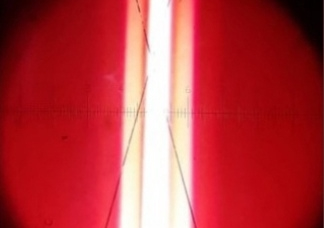
\includegraphics[width=9cm]{exp6}\\
\textit{рис.7 Дифракционная картинка на частоте $\nu = 1,477$ Мгц}\\
\\
2.3) \begin{tabular}{|l|l|l|l|}
\hline
m & -1 & 0 & 1\\
\hline
$x_m$, мкм & 1980 & 1720 & 1460\\
\hline
\end{tabular}\\
\\
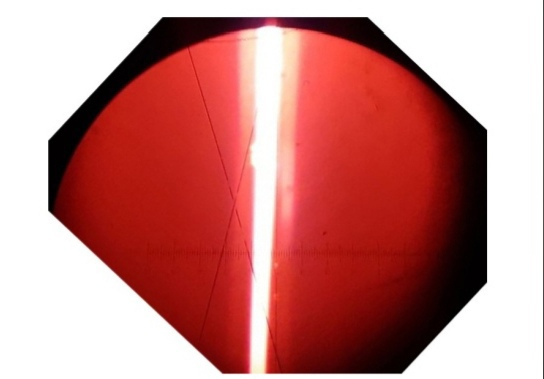
\includegraphics[width=9cm]{exp7}\\
\textit{рис.8 Дифракционная картинка на частоте $\nu = 2,106$ Мгц}\\
\\
3) Для каждой из трёх частот построим график зависимости координаты $x_m$ от порядка $m$ и по наклону прямой определим расстояние между соседними полосами: $$\frac{l_m}{m} = \frac{\Delta x_m}{\Delta m} = \tg \alpha$$
Рассчитаем длину $\Lambda$ УЗ-волны по формуле (4), а скорость ультразвука по формуле (5).
Результаты занесём в таблицу:\\
\begin{center}
\begin{tabular}{|l|l|l|l|}
\hline
$\nu$, МГц & 1,115 & 1,477 & 2,106\\
\hline
$\tg \alpha$, мкм & 134 & 180 & 260\\
\hline
$\sigma_{\tg \alpha}$, мкм & 10 & 10 & 10\\
\hline
$\Lambda$, мм & 1,35 & 1,01 & 0,70\\
\hline
$\sigma_{\Lambda}$, мм & 0,07 & 0,05 & 0,03\\
\hline
$v$, м/с & 1510 & 1489 & 1470\\
\hline
$\sigma_v$, м/с & 76 & 75 & 74\\
\hline
\end{tabular}\\
\end{center}
4) Таким образом, скорость ультразвука в воде по результатам экспериментов получилась:
$$v_{exp} \approx (1490 \pm 110) \; \textit{м/с}$$
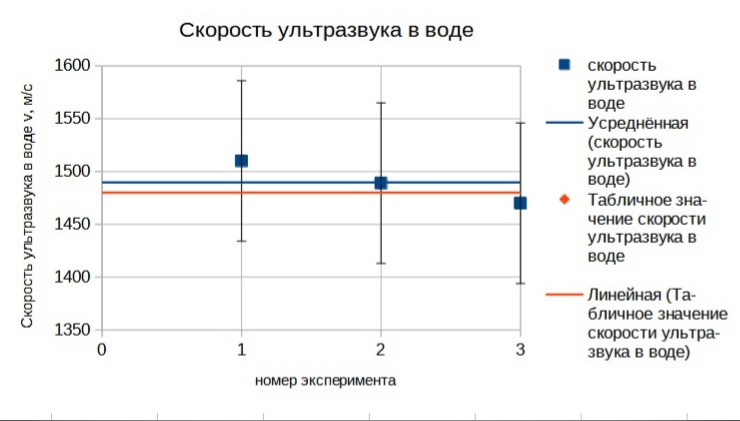
\includegraphics[width=9cm]{g2}\\
\textit{рис.10 Результаты эксперимента и среднее экспериментальное значение скорости ультразвука в воде}\\
\item \textbf{Определение скорости ультразвука методом тёмного поля}\\
5) Соберем схему, изображенную на рисунке 4. Найдем цену деления шкалы микроскопа для последующих измерений: $\delta = 0,048 \; \textit{мм}$. \\
После закрытия нулевого максимума остаточное поле:
\begin{equation}\label{trivial}
f(x) = \frac{im}{2}\exp^{i\Omega x} + \frac{im}{2}\exp^{-i\Omega x}= im\cos \Omega x
\end{equation}
Картина интенсивности:
\begin{equation}\label{trivial}
I(x) = m^2 \cos^2 \Omega x
\end{equation}\\
\end{enumerate}
\end{enumerate}
\end{multicols}
\begin{center}
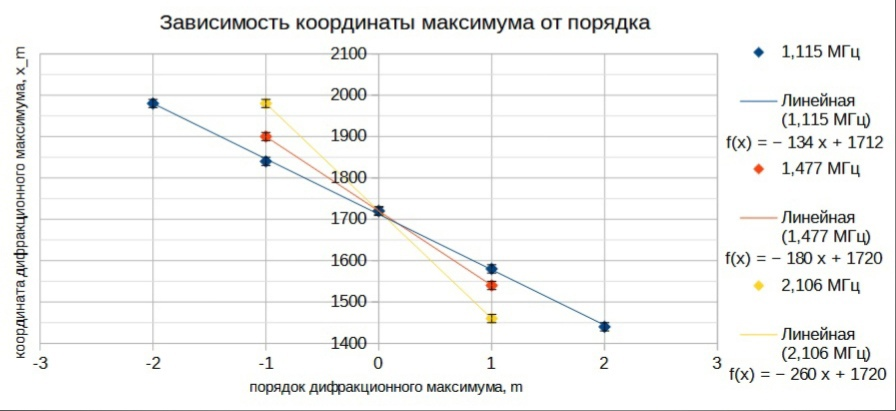
\includegraphics[width=14cm]{g1}\\
\textit{рис.9 Зависимость координаты максимума от порядка для различных частот}\\
\end{center}
\begin{multicols}{2}
\small
6) После закрытия проволокой центрального максимума определяем координаты первой $x_1$ и последней $x_2$ хорошо видимых полос и количество светлых промежутков между ними $n$.
Картины наблюдения получились только при частотах
$$\nu_1 = 0,819 \; \textit{МГц} \; \; \; \nu_2 = 1,052 \; \textit{МГц}$$
Определим для этих данных скорость звука и длину волны:
\begin{center}
\footnotesize
\begin{tabular}{|c|c|c|c|c|c|}
			\hline
			 $\nu$, МГц & $x_1$, мм & $\sigma_{x_1}$, мм & $x_2$, мм & $\sigma_{x_2}$, мм & n  \\ \hline
			 1,052 & 0,029 & 0,05 & 1,651 & 0,05 & 10  \\ \hline
			0,819 & 0,038 & 0,05 & 1,699 & 0,05 & 13  \\ \hline
		\end{tabular}
\end{center}
\small
C помощью формул (4) и (5) определим скорость ультразвука в воде методом тёмного поля:
\begin{center}
\begin{tabular}{|c|c|c|c|c|}
			\hline
			$\nu$, МГц & $l_m$, мм & $\Lambda$, мм &  $v$, м/с & $\sigma_{v}$, м/с  \\ \hline
			1,052 & 0,16  & 1,1  & 1190 & 370  \\ \hline
			0,819 & 0,13 & 1,4  & 1140 & 440  \\ \hline
		\end{tabular}
\end{center}
Таким образом, скорость ультразвука в воде, измеренная с поомщью метода темного поля, получилась:
$$v_{exp} \approx (1160 \pm 440) \; \textit{м/с}$$
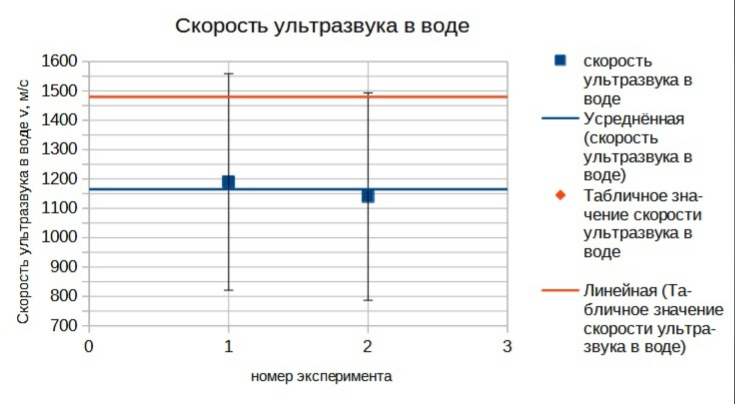
\includegraphics[width=9cm]{g3}\\
\textit{рис.11 Результаты эксперимента по методу тёмного поля}\\
\indent 5. \textbf{Заключение}\\
В данной работе было изучено явление дифракции света на синусоидальной акустической решётке, а также наблюдалась фазовая решётка с помощью метода тёмного поля. Для двух экспериментов была вычислена скорость ультразвука в воде. Экспериментальные значения сходятся с теоретическими в пределах погрешности.\\
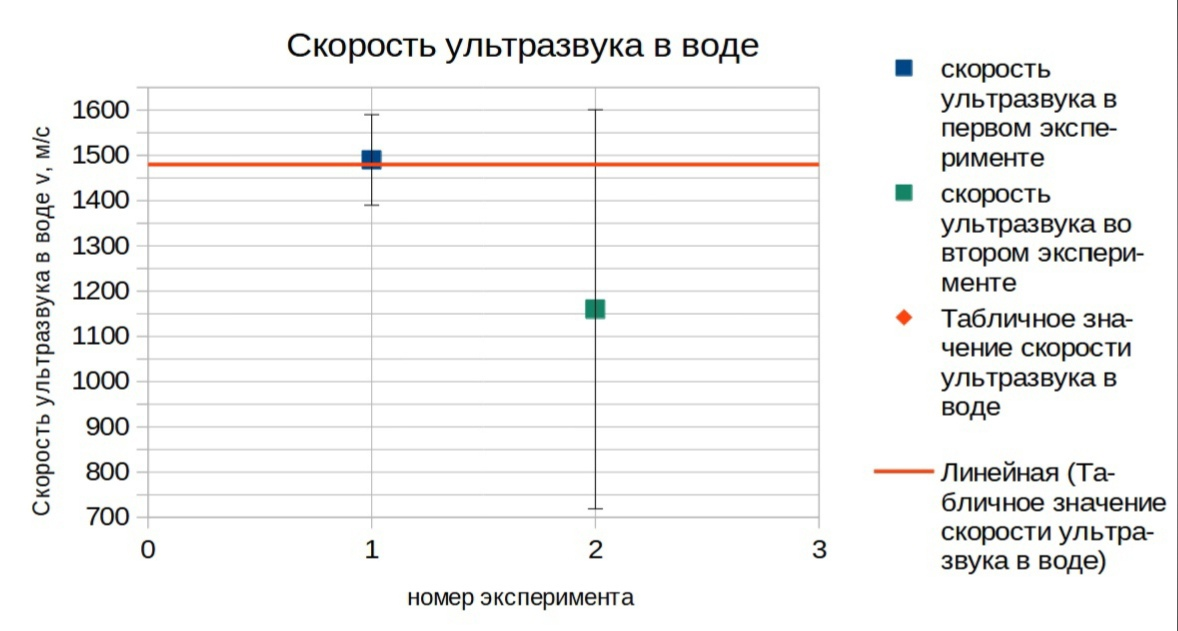
\includegraphics[width=9cm]{g4}\\
\textit{рис.12 Значения скорости ультразвука в воде для двух опытов}\\
\\
\textit{1. Общий курс физики. Оптика, Д.В.Сивухин}\\
\textit{2. Лабораторный практикум по общей физике. Оптика, А.В. Максимычев}\\
\end{multicols}
\end{document}